\section*{Exercice 8~: L'utilisation des réseaux de Pétri pour le
  contrôle des trains}

\subsection*{Question 1}

Chaque place pourra correspondre à un secteur, chaque jeton à un train et chaque
transition et un movement de train d'un secteur à la prochaine~:

\begin{center}
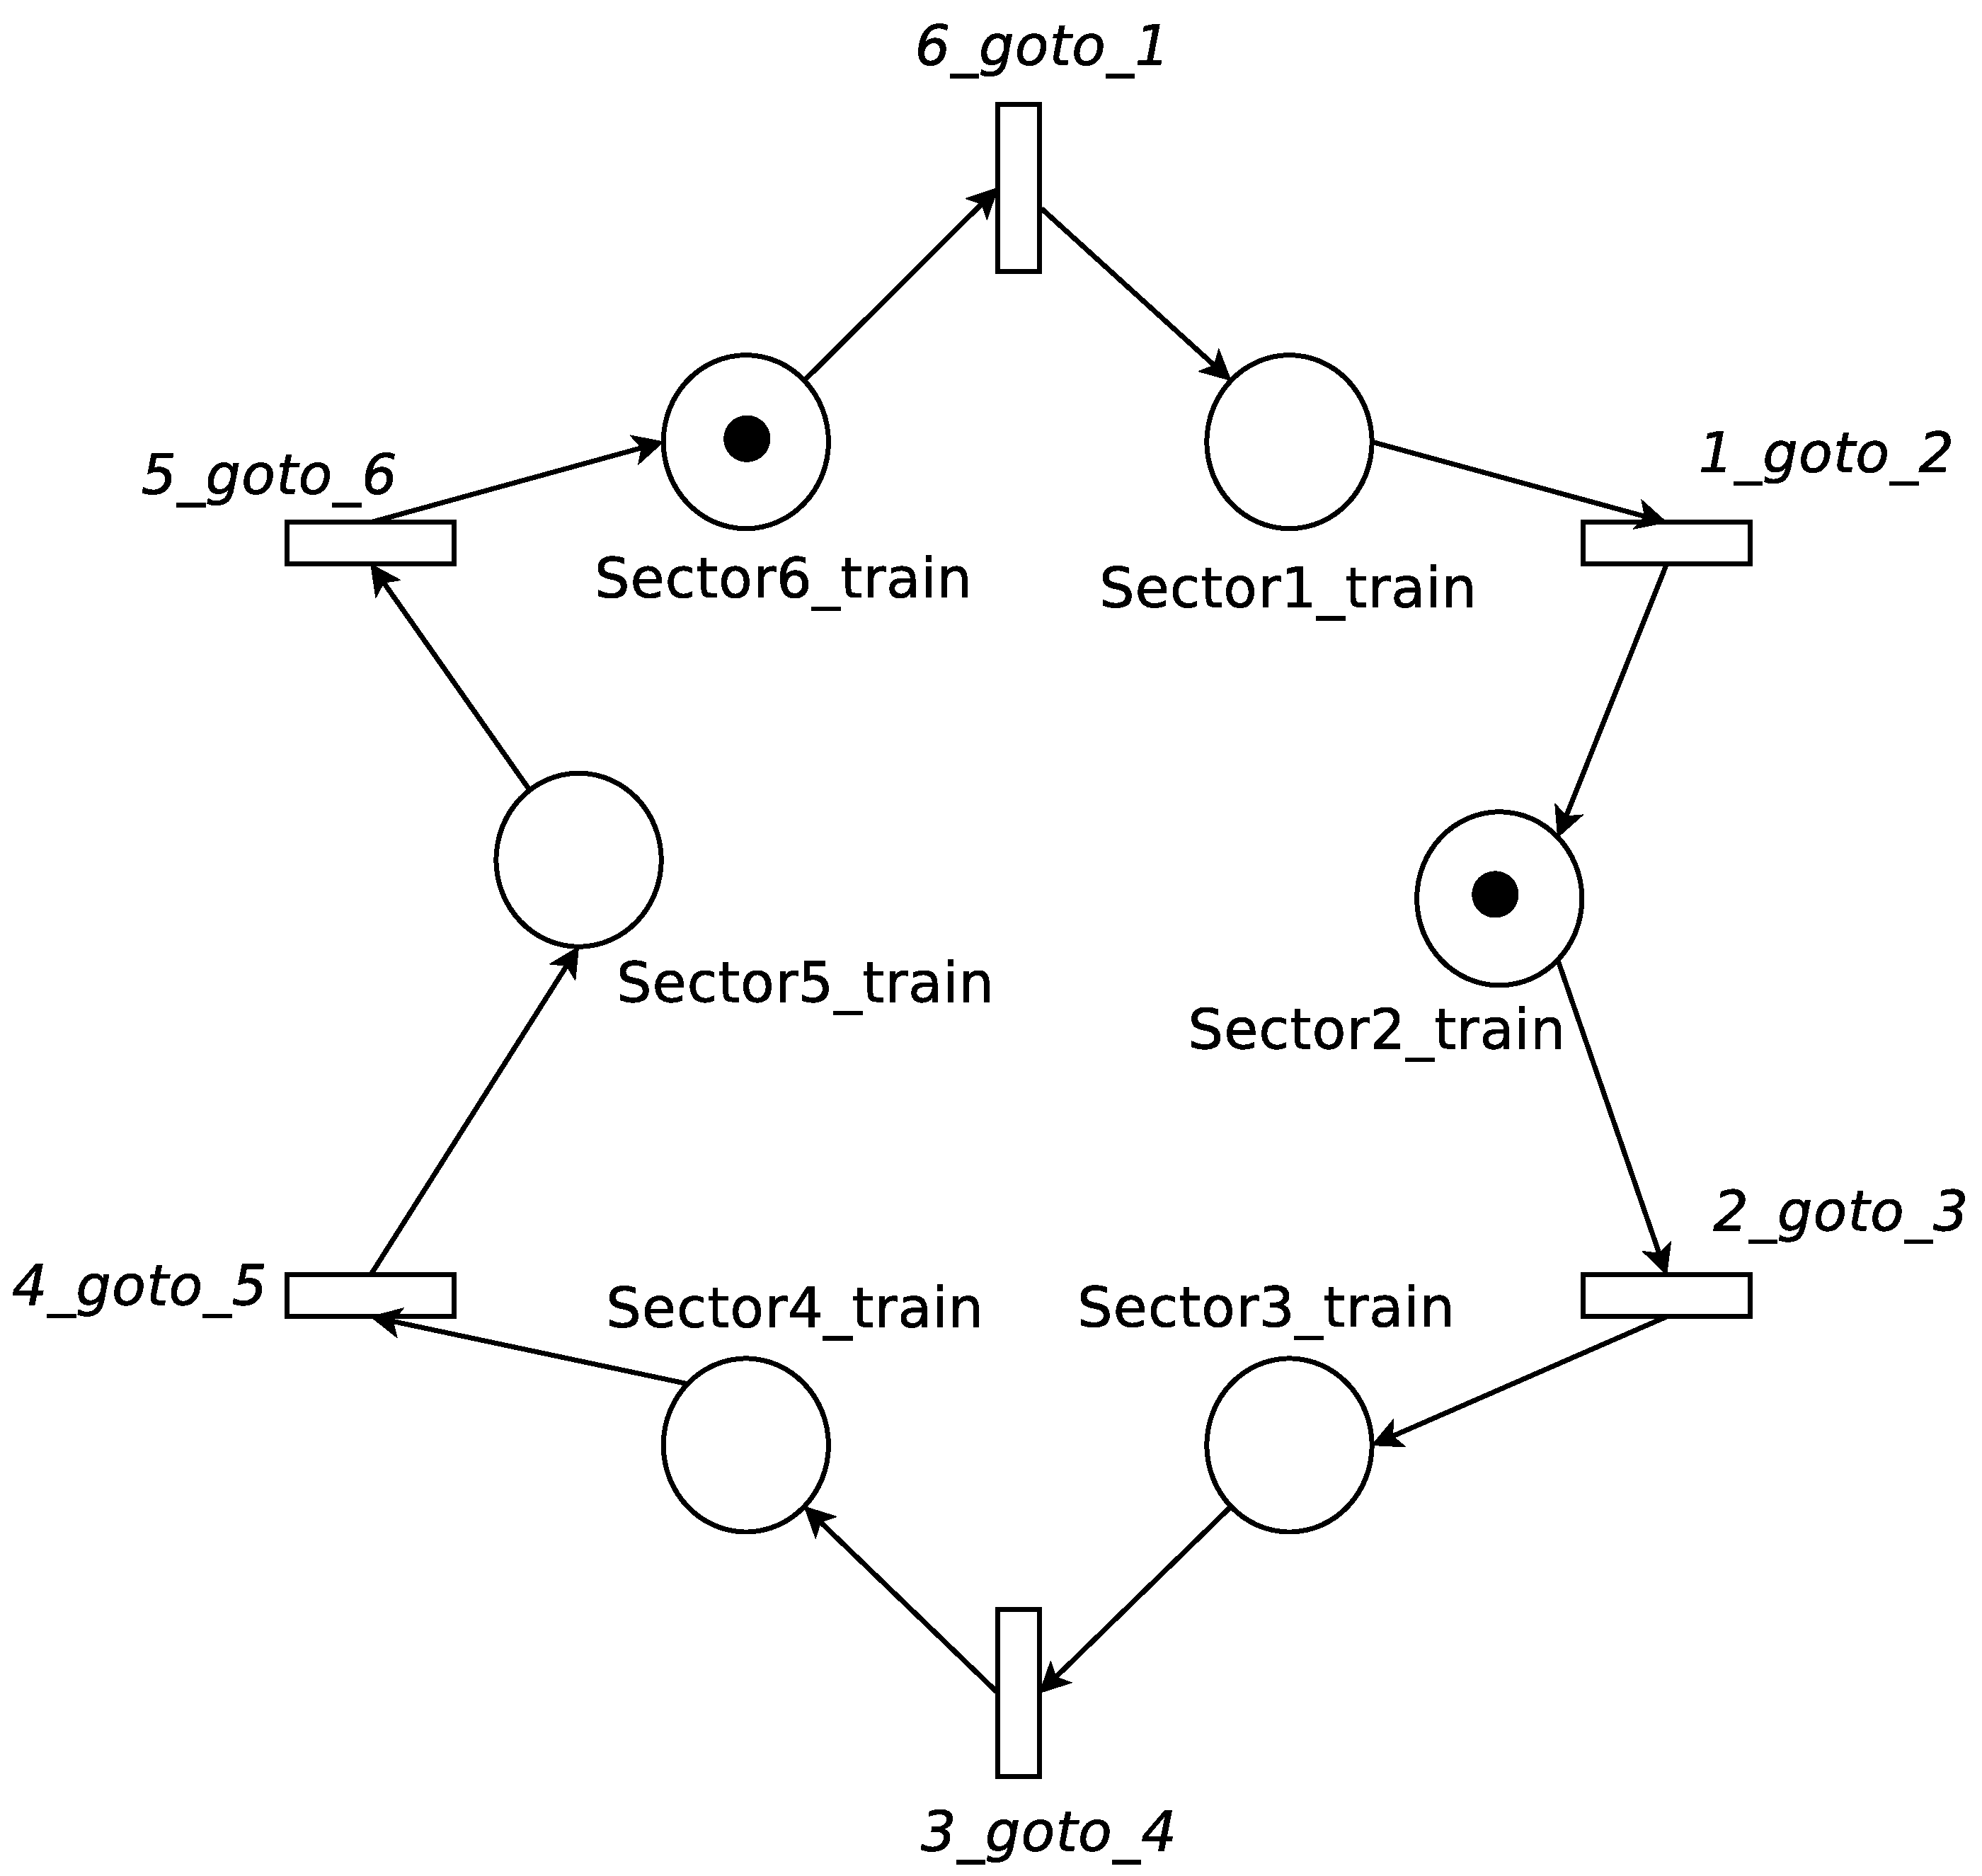
\includegraphics[height = 0.3\paperwidth]{exo8_1.eps}
\end{center}

Le réseau ci-dessus n'empêche cependant pas la collision de trains, choses qu'il 
serait préférable d'éviter. Démunies d'arcs inhibiteurs, nous devions créer pour 
chaque secteur une place binaire dont la présence d'un jeton correspond à la non 
présence de train dans ce secteur.

\emph{Les parties ajoutées sont en vert~:}

\begin{center}
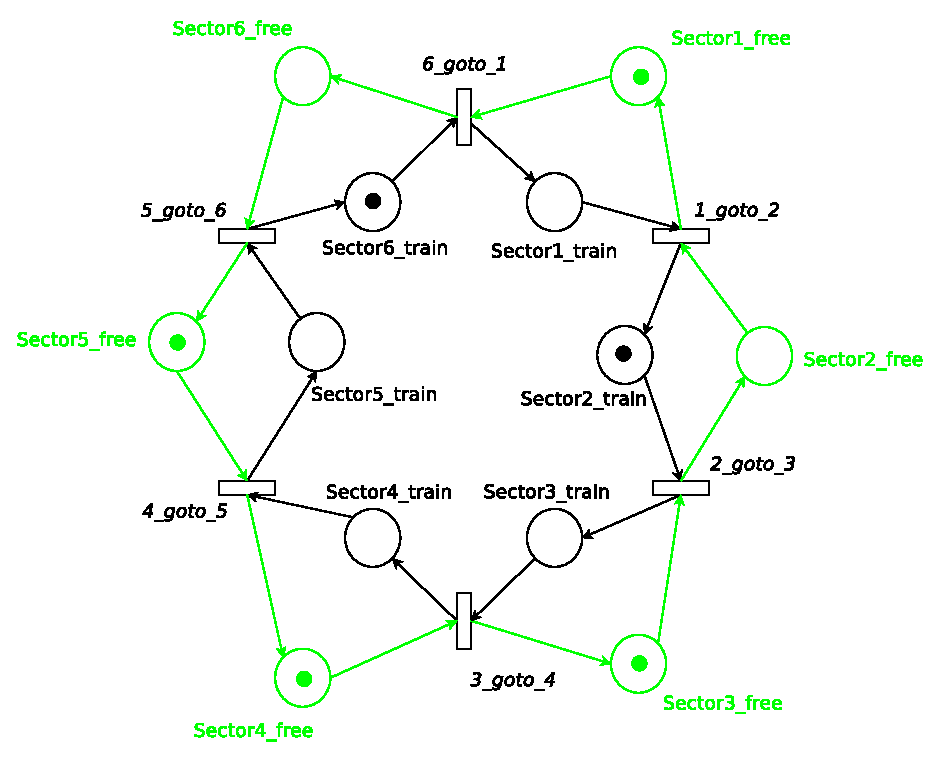
\includegraphics[height = 0.4\paperwidth]{exo8_2.eps}
\end{center}

Nous avons ainsi comme invariants qu'un secteur est toujours soit libre, soit
occupé par un seul et unique train. Il nous reste comme condition à remplir que
les secteurs adjascentes à un secteur occupé soient libres~:

\begin{center}
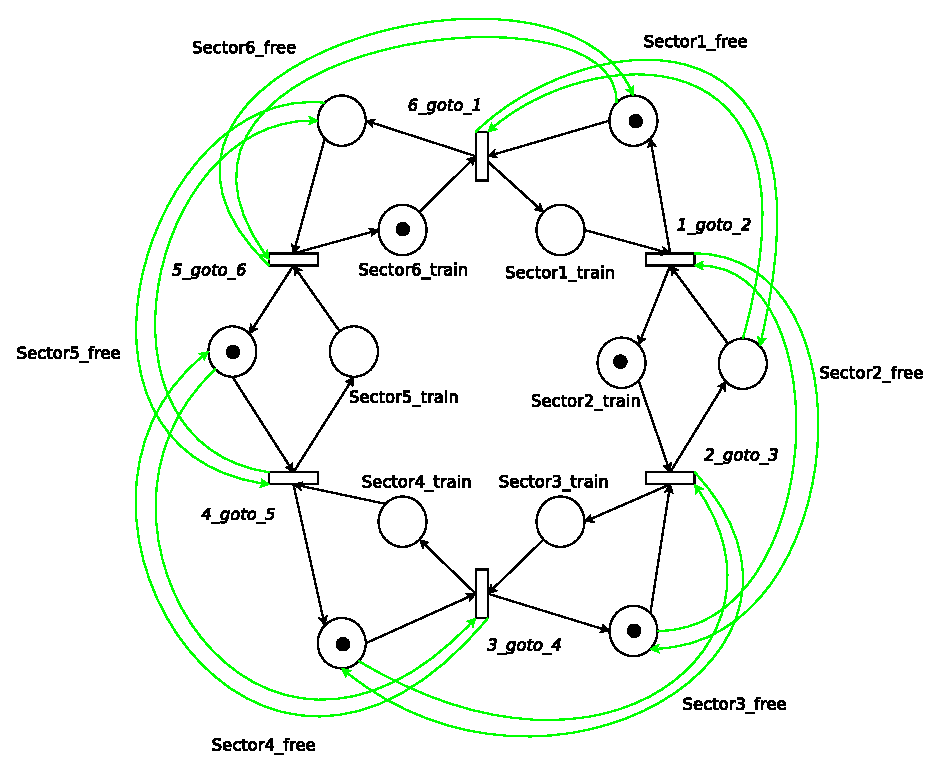
\includegraphics[height = 0.5\paperwidth]{exo8_3.eps}
\end{center}

Maintenant il faut différencier les deux trains, choses que nous pouvions faire
en recopiant le cycle interne de places. 

\emph{Pour faciliter la lecture, les deux circuits analogiques pour le deux trains ont
étés coloriés en rouge et en bleu respectivement~:}

\begin{center}
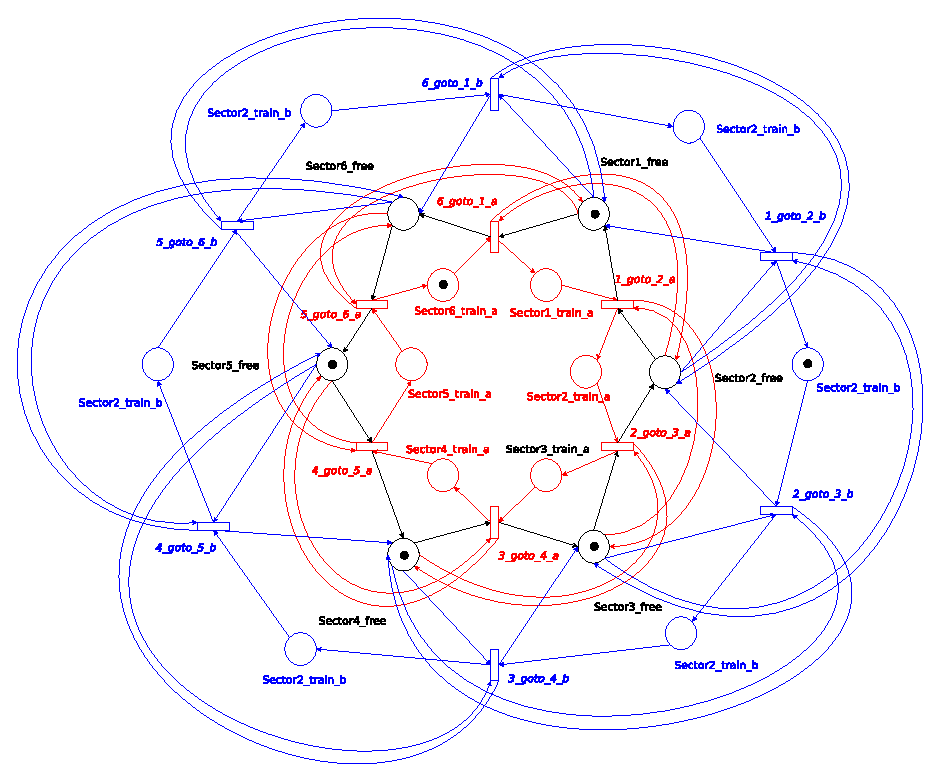
\includegraphics[height = 0.6\paperwidth]{exo8_uncoloured.eps}
\end{center}


\subsection*{Question 2}

En parant du réseau précendant et en écrasant les deux circuits \og{}train\fg{}
en un seule, nous nous retrouvons avec le réseau colorié suivant.

\emph{Le jeton rouge représente le premier train, le bleu la deuxième, et ceux
noirs l'absence de train pour un secteur donné~:}

\begin{center}
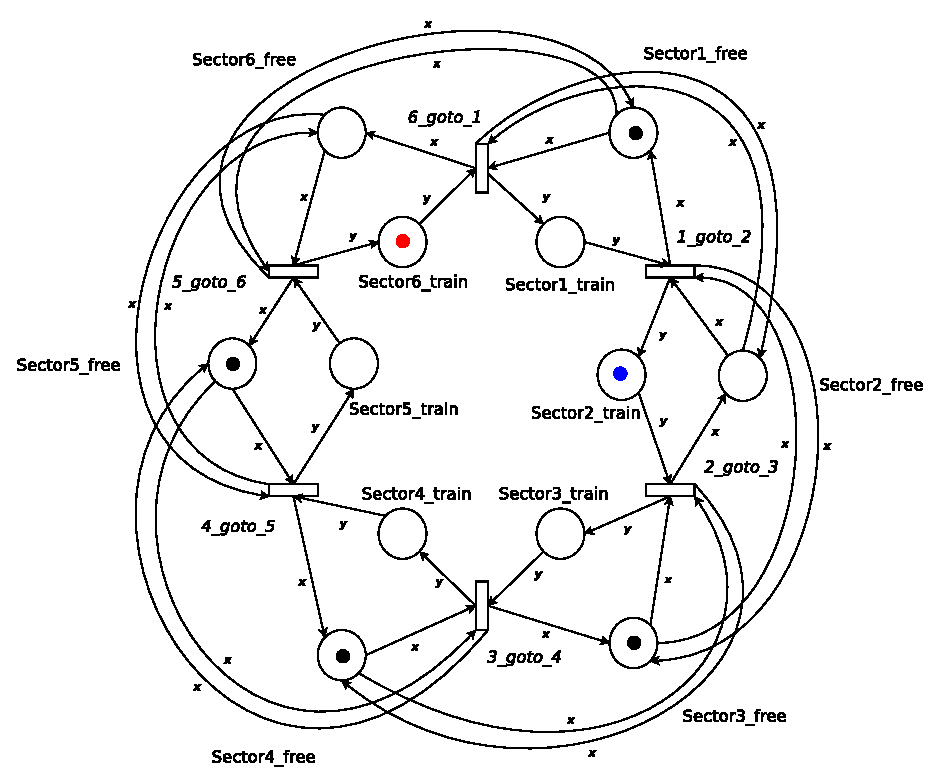
\includegraphics[height = 0.5\paperwidth]{exo8_coloured.eps}
\end{center}

Il est possible de simplifier ce réseau en écrasant les deux cycles ensemble. 
Ci-dessous un jeton noir correspond à la non-présence d'un train dans le secteur 
correspondant, un jeton d'une autre couleur à un train présent~:

\begin{center}
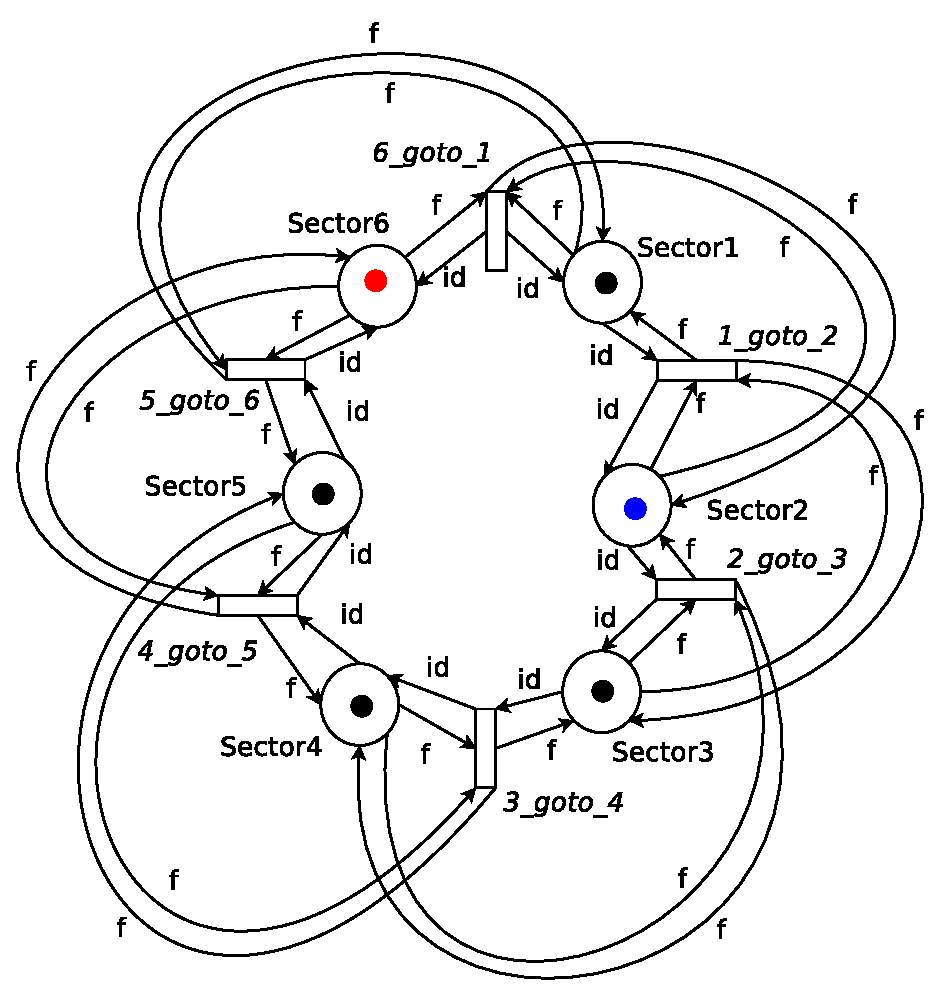
\includegraphics[height = 0.5\paperwidth]{exo8_coloured_2_v2.eps}
\end{center}

Où~:

$\forall c \in \{RED, BLUE\}$ $id(c) = c$

$\forall c \in \{RED, BLUE\}$ $f(c) = BLACK$

Ce réseau est beaucoup plus simple à aborder que la version non-coloré, qui pour
$n$ trains aura $n+1$ fois plus de places. Celà étant sans la définition de la
fonction $f$ (projection dans le noir) il n'est pas possible de comprendre le 
fonctionnement du réseau. 

Le premier réseau coloré est un bon compromis entre les deux~: il a du sens sans
information supplémentaire, mais reste un facteur linéaire plus compacte que le 
réseau non-coloré.


\subsection*{Question 3}
